\documentclass[25pt, a0paper, portrait]{tikzposter}
\usepackage[utf8]{inputenc}
\usepackage{blindtext}
\usepackage{comment}
\usepackage{float}                                                                                        
\usepackage{amsmath} %for \text{}                                                                         
\usepackage{amssymb}                                                                                      
\usepackage{graphicx}                                                                                     
\usepackage[toc,page]{appendix}                                                                           
\usepackage{geometry}                                                                                     
\usepackage{eufrak}                                                                                       
\usepackage{fixltx2e}                                                                                     
\usepackage{bm}                                                                                           
\usepackage{tikz}                                                                                         
\usepackage{float}                                                                                        
\usepackage{xcolor}   

\makeatletter
\def\title#1{\gdef\@title{\scalebox{\TP@titletextscale}{%
\begin{minipage}[t]{\linewidth}
\centering
#1
\par
\vspace{0.5em}
\end{minipage}%
}}}
\makeatother
 
\title{Reformulation, Extension, and Application
\newline of the Formal Framework for P Systems}
\author{Ren Tristan A. de la Cruz}
\date{\today}
\institute{University of the Philippines - Diliman}
 
%\usetheme{Autumn}
\begin{document}
 
\maketitle

\begin{columns}
\column{0.4} 
\block{Abstract}
{
\emph{Membrane computing} is a field of computer science that studies biologically-inspired          
parallel and distributed models of computations known as \emph{P systems}. At the moment, there      
are hundreds of P systems variants with their own syntax and often informally defined semantics.     
\emph{Formal framework} attempts to formally define a general syntax and procedural semantics for    
wide variety of P systems. This research proposal is about the reformulation, extension, and         
application of the said formal framework. 
}
\column{0.6}
\block{P Systems}
{
The term `\textit{P systems}' refers to a family of           
models of computation which are inspired by biological processes. P system models use abstractions        
of biological processes as computational operations. For example, different types of rules                
(operations) used by most P system variants are abstractions of processes like \textit{chemical           
reaction} and \textit{ion transport} that occur inside biological cells. Most P system variants use       
\textit{object symbols} as the objects of computation. One can think of these object symbols as           
abstraction of physical \textit{molecules} or \textit{ions}. P systems store \textit{multisets} of        
these object symbols inside regions enclosed by \textit{membranes}. A P system has a collection of        
these membranes with multisets of objects symbols inside. The membranes can be `connected' to each        
other to form a \textit{membrane structure}.                                                              
}
\end{columns}

\begin{columns}

   \column{0.20}
   \block{Tree Structure}
   {
   \begin{tikzfigure}                                                                                  
   \begin{center}                                                                                       
   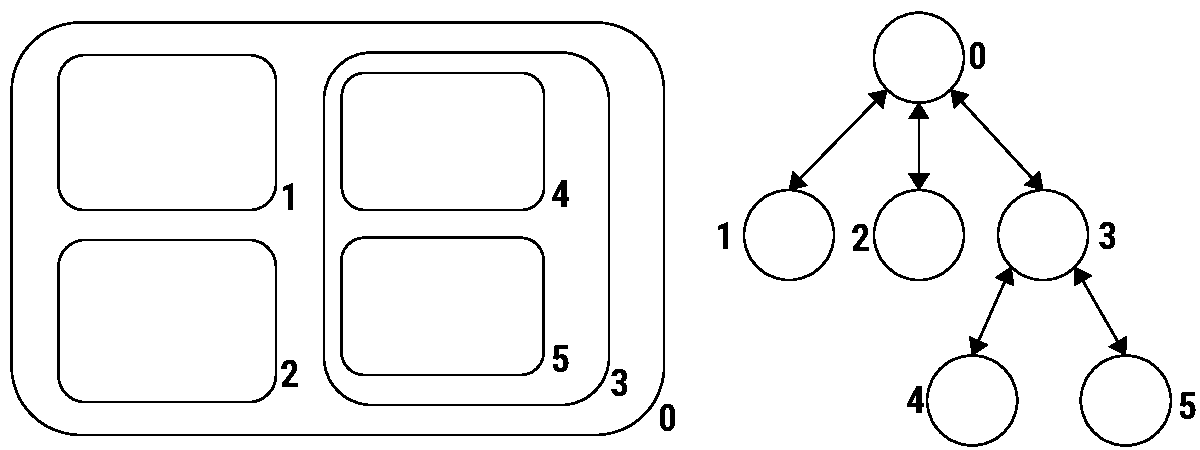
\includegraphics[scale=0.65]{figures/zzz-cell-like-structure.pdf}                                    
   \label{fig:cell-like}                                                                                
   \end{center}                                                                                         
   \end{tikzfigure}   
   }

   \column{0.20}
   \block{Graph Structure}
   {
   \begin{tikzfigure}
   \begin{center}                                                                                       
   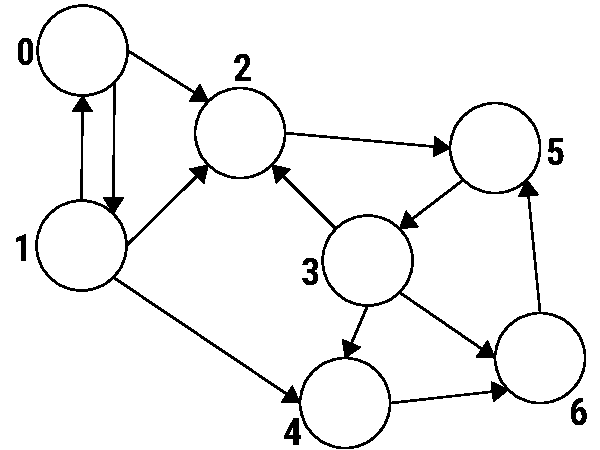
\includegraphics[scale=0.65]{figures/zzz-graph-topology.pdf}                                         
   \label{fig:graph-topology}                                                                           
   \end{center}                                                                                         
   \end{tikzfigure} 
   }

   \column{0.30}
   \block{Multiset on Membranes}
   {
   \begin{tikzfigure}                                                                                   
   \begin{center}                                                                                       
   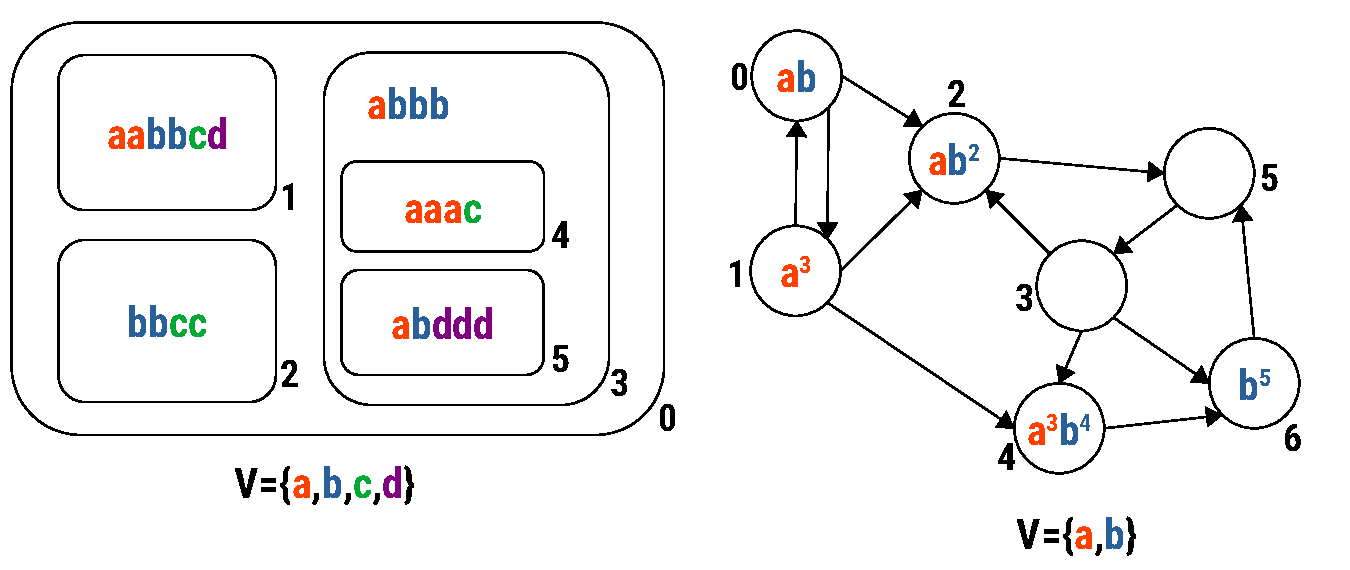
\includegraphics[scale=0.70]{figures/zzz-multisets-on-membranes.pdf}                                 
   \label{fig:multisets-on-membranes}                                                                   
   \end{center}                                                                                         
   \end{tikzfigure}     
   }

   \column{0.30}
   \block{Rewriting Rule}
   {
   \begin{tikzfigure}                                                                                    
   \begin{center}                                                                                       
   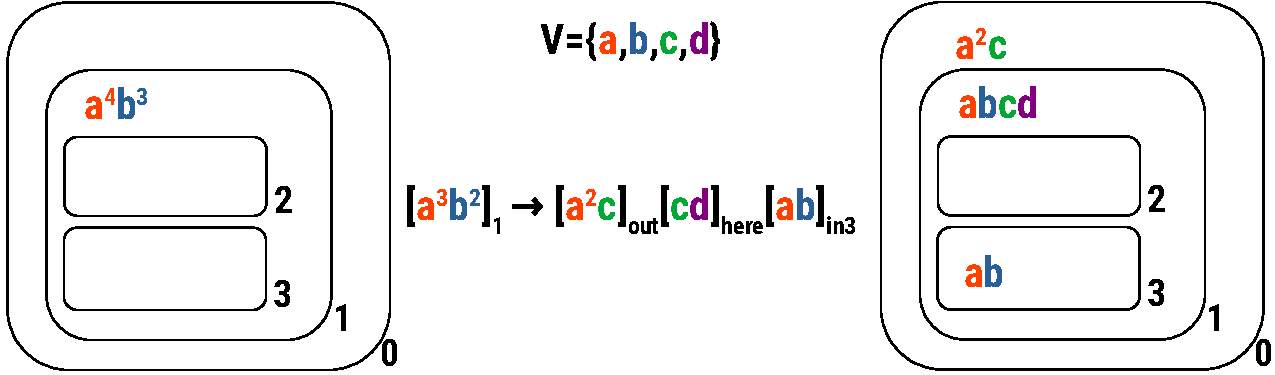
\includegraphics[scale=1.0]{figures/zzz-transition-rule.pdf}                                        
   \label{fig:trans-rule}                                                                               
   \end{center}                                                                                         
   \end{tikzfigure}  
   }
\end{columns}

\begin{columns}


   \column{0.3333}
   \block{Rule with Dissolution}
   {
   \begin{tikzfigure}                                                                                    
   \begin{center}                                                                                       
   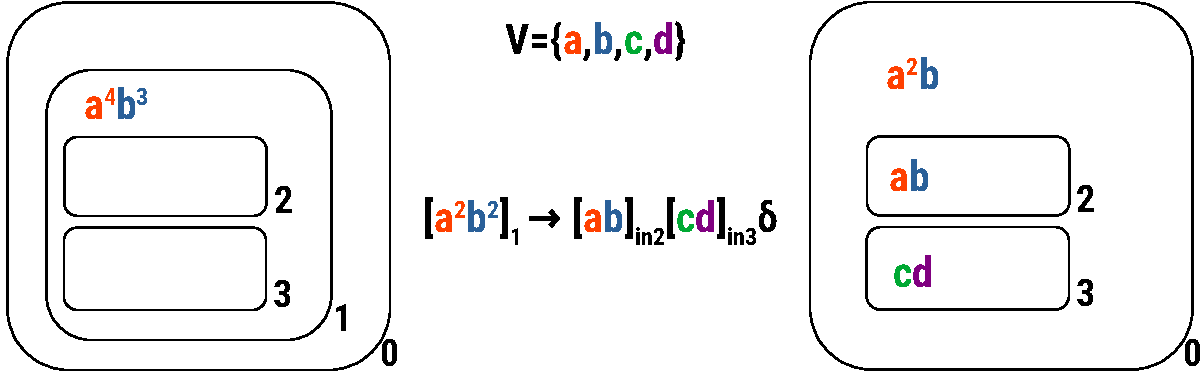
\includegraphics[scale=1.2]{figures/zzz-transition-rule2.pdf}                                       
   \label{fig:trans-rule2}                                                                              
   \end{center}                                                                                         
   \end{tikzfigure}
   }

   \column{0.3333}
   \block{Tissue P Rules}
   {
   \begin{tikzfigure}                                                                                   
   \begin{center}                                                                                       
   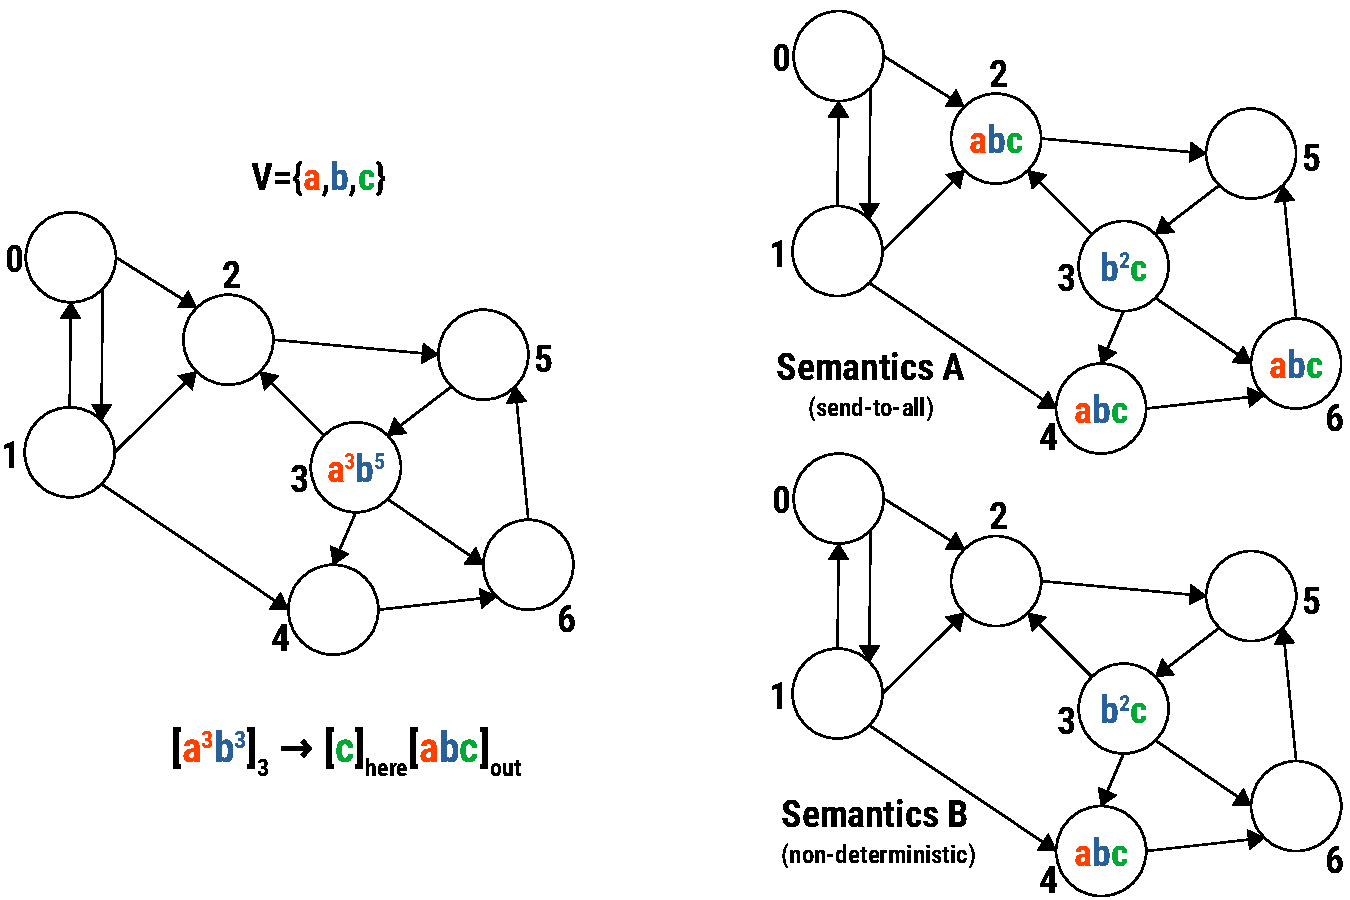
\includegraphics[scale=0.60]{figures/zzz-tissue-rule.pdf}                                            
   \label{fig:tissue-rule}                                                                              
   \end{center}                                                                                         
   \end{tikzfigure}     
   }

   \column{0.3333}
   \block{Active Membranes}
   {
   \begin{tikzfigure}                                                                                    
   \begin{center}                                                                                       
   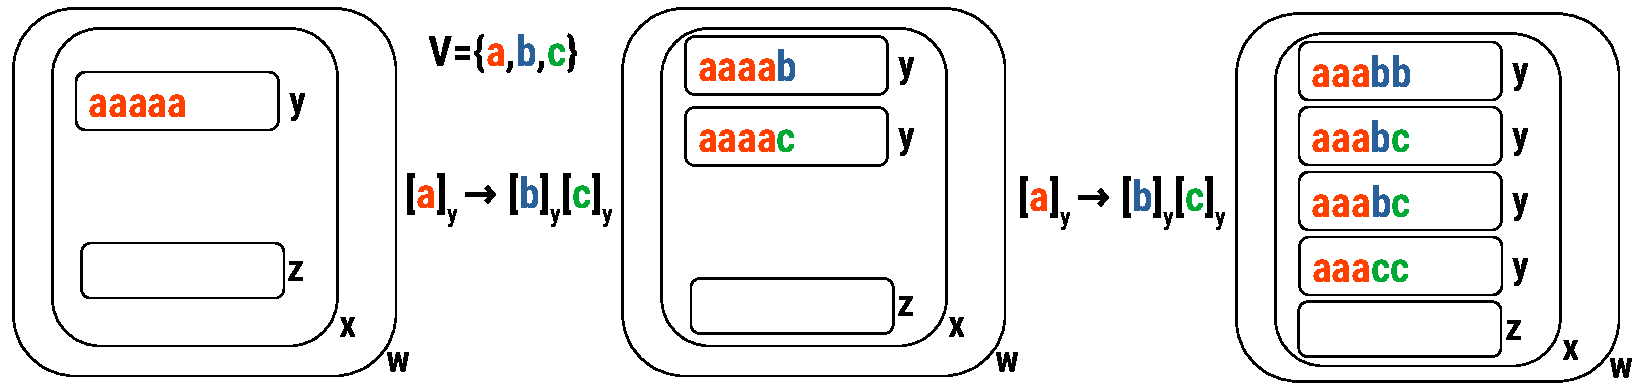
\includegraphics[scale=0.85]{figures/zzz-active-mem-rule.pdf}                                        
   \label{fig:active-mem-rule}                                                                          
   \end{center}                                                                                         
   \end{tikzfigure}   
   }
\end{columns}

\block{Formal Framework}
{
There are tens, if not hundreds, of P system variants. Their syntax are well-defined but the         
semantics are often described in an informal manner. \emph{Formal framework} is an attempt to        
formalize not only syntax but also the procedural semantics of a wide variety of P systems. There    
are currently three versions of the framework, (FF1) one for P systems with static membrane structures,      
(FF2) one for P systems with dynamic membrane structures, and (FF3) another for static P systems with            
input-output. The formal frameworks can be used to analyze, compared, and extended P systems. 
}

\begin{columns}
   \column{0.7}
   \block{Proposal}
   {
      The research proposal has three aspects: (1) the reformulation of the formal framework, (2) the      
      extension of the formal framework, and (3) the application of the formal framework.            
      Reformulating the formal framework means changing the framework by changing the notions/concepts     
      used or using different formalizations for these notions but not affecting the usefulness of the     
      framework. Extending the framework means adding new notions and formalizations to extended the       
      scope or usefulness of the framework. An extended framework can mean it can model more P system      
      variants or that there are more notions in the framework that can provide more insights to the       
      workings of existing `supported' P system variants. Application of the framework means using the     
      framework to analyze, compare, and/or extended existing P system variants.  
   }
   \column{0.3}
   \block{Aspects}
   {
      \begin{tikzfigure}                                                                                    
      \begin{center}                                                                                       
      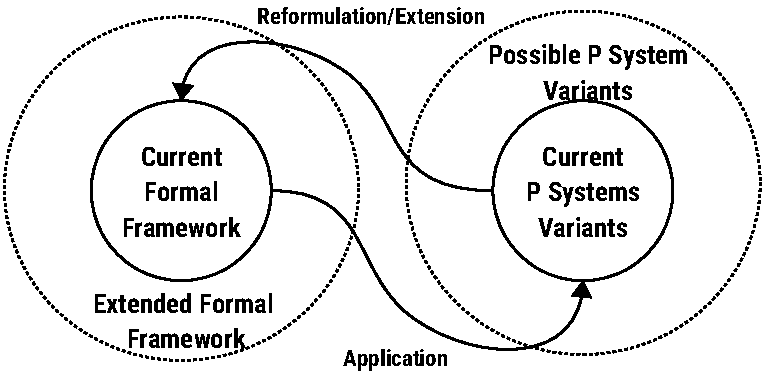
\includegraphics[scale=1.25]{figures/zzz-ff-p-system.pdf}                                            
      \label{fig:ff-p-system}                                                                              
      \end{center}                                                                                         
      \end{tikzfigure}                                                                                         
   }
\end{columns}



\begin{columns}


\column{0.65}
\block{Objectives}
{
\begin{enumerate}                                                                                    
   \item (Reformulation) Combine FF2 and FF3 into a single formal framework. The purpose of this objective is to have a single formal framework (FF)        
         that can be used of static or dynamic P systems.                                                 
   \item (Reformulation) Reformulate the interaction rule in FF (from objective 1) in a                   
         \emph{bottom-up} manner instead of the \emph{top-down} approach of the FF. The rule in the       
         FF (or specifically FF2) contains 11 components because it is trying to be the most general      
         and unrestricted version of a rule such that the rule types from the P system variants are  
         simply restricted versions of the more general FF interaction rule. We call this approach   
          \emph{top-down}. A rule    
         can instead be defined as a `combination' of simpler `elementary' rules. We start from the  
         \emph{bottom} with this `elementary' rules and use them to define a general rule which is   
         a combination of these `elementary' rules.                                                  
   \item (Application) Perform a comprehensive survey of the different P system variants and use the 
         FF to create the equivalent FF models of the different P system variants.                   
   \item (Extension) While doing the comprehensive survey of P system variants, if there are         
         variants that are difficult or impossible to create an FF model for, formalize the features 
         of these variants and use them to extended the FF.                           
   \item (Application) Create a simulator for FF models. Combining this simulator with the FF models 
        of the P systems from the survey (objective 4) will result in a fairly general simulator     
        than can simulate a wide variety of P systems.                                               
\end{enumerate}   

}


\column{0.35}
\block{Timeline}
{
   \begin{tikzfigure}
   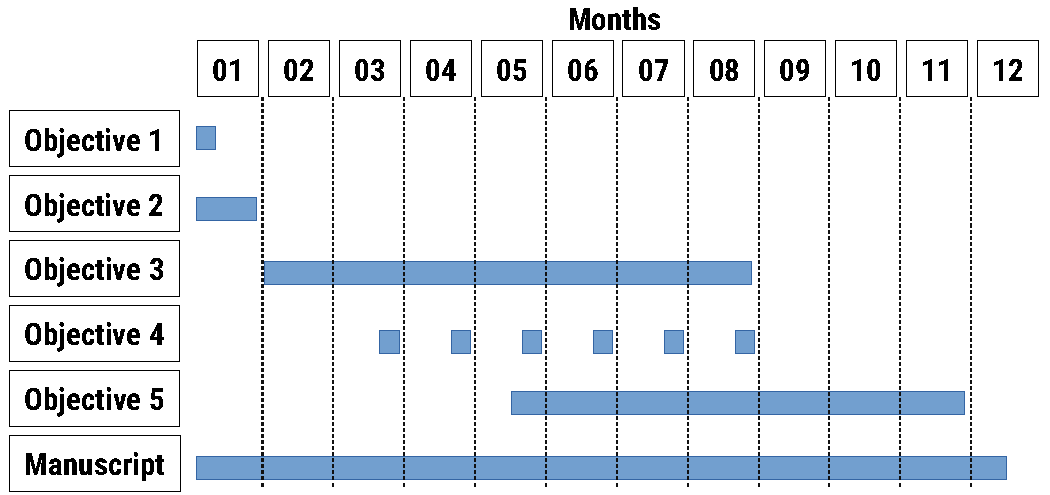
\includegraphics[scale=1.3]{figures/zzz-schedule.pdf}
   \end{tikzfigure}
}

\end{columns}
 
\end{document}

